% !TEX TS-program = pdflatex
% !TEX encoding = UTF-8 Unicode

% This is a simple template for a LaTeX document using the "article" class.
% See "book", "report", "letter" for other types of document.

\documentclass[12pt]{article} % use larger type; default would be 10pt
\usepackage[utf8]{inputenc}   % set input encoding (not needed with XeLaTeX)

%%% PAGE DIMENSIONS
\usepackage{geometry}
\geometry{letterpaper}
\geometry{margin=1in} % 1in page margin

%%% COLOR AND GRAPHICS
\usepackage{color}
\usepackage{graphicx} % support the \includegraphics command and options

\usepackage{pslatex}
\definecolor{mygreen}{rgb}{0,0.6,0}
\definecolor{mygray}{rgb}{0.5,0.5,0.5}
\definecolor{mymauve}{rgb}{0.58,0,0.82}
\usepackage{listings} % For displaying source code
\lstset{ %
	language=C,                      % the language of the code
	backgroundcolor=\color{white},   % choose the background color; you must add \usepackage{color} or \usepackage{xcolor}
	basicstyle=\sffamily\fontsize{11}{13.2}\selectfont,        % the size of the fonts that are used for the code
	breakatwhitespace=false,         % sets if automatic breaks should only happen at whitespace
	breaklines=true,                 % sets automatic line breaking
	captionpos=t,                    % sets the caption-position to bottom
	commentstyle=\color{mygreen},    % comment style
	deletekeywords={...},            % if you want to delete keywords from the given language
	escapeinside={\%*}{*)},          % if you want to add LaTeX within your code
	extendedchars=true,              % lets you use non-ASCII characters; for 8-bits encodings only, does not work with UTF-8
	frame=single,                    % adds a frame around the code
	keepspaces=true,                 % keeps spaces in text, useful for keeping indentation of code (possibly needs columns=flexible)
	keywordstyle=\color{blue},       % keyword style
	morekeywords={*,...},            % if you want to add more keywords to the set
	numbers=left,                    % where to put the line-numbers; possible values are (none, left, right)
	numbersep=5pt,                   % how far the line-numbers are from the code
	numberstyle=\color{mygray},      % the style that is used for the line-numbers
	rulecolor=\color{black},         % if not set, the frame-color may be changed on line-breaks within not-black text (e.g. comments (green here))
	showspaces=false,                % show spaces everywhere adding particular underscores; it overrides 'showstringspaces'
	showstringspaces=false,          % underline spaces within strings only
	showtabs=false,                  % show tabs within strings adding particular underscores
	stepnumber=1,                    % the step between two line-numbers. If it's 1, each line will be numbered
	stringstyle=\color{mymauve},     % string literal style
	tabsize=2,                       % sets default tabsize to 2 spaces
	title=\lstname                   % show the filename of files included with \lstinputlisting; also try caption instead of title
}

% \usepackage[parfill]{parskip} % Activate to begin paragraphs with an empty line rather than an indent

%%% PACKAGES
\usepackage{booktabs} % for much better looking tables
\usepackage{array}    % for better arrays (eg matrices) in maths
\usepackage{paralist} % very flexible & customisable lists (eg. enumerate/itemize, etc.)
\usepackage{verbatim} % adds environment for commenting out blocks of text & for better verbatim
%\usepackage{subfig}   % make it possible to include more than one captioned figure/table in a single float
\usepackage{subcaption}
\usepackage{adjustbox}
\usepackage{placeins} % allows for use of \FloatBarrier to prevent floats from moving past line.

%%% HEADERS & FOOTERS
%\usepackage{fancyhdr} % This should be set AFTER setting up the page geometry
%\pagestyle{fancy} % options: empty , plain , fancy
%\renewcommand{\headrulewidth}{0pt} % customise the layout...
%\lhead{}\chead{}\rhead{}
%\lfoot{}\cfoot{\thepage}\rfoot{}


%%% SECTION TITLE APPEARANCE
\usepackage{sectsty}
\sectionfont{\normalsize\bfseries\uppercase}
\subsectionfont{\normalsize\bfseries}
\subsubsectionfont{\normalsize\mdseries\itshape}

%%% ToC (table of contents) APPEARANCE
\usepackage[nottoc,notlof,notlot]{tocbibind} % Put the bibliography in the ToC
\usepackage[titles]{tocloft} % Alter the style of the Table of Contents
\renewcommand{\cftsecfont}{\rmfamily\mdseries\upshape}
\renewcommand{\cftsecpagefont}{\rmfamily\mdseries\upshape} % No bold!

%%% Title setup
\newcommand{\TitleFont}{\fontsize{16}{20}\selectfont\bfseries}
\newcommand{\AuthorFont}{\fontsize{14}{17}\selectfont}

%%% END Article customizations

%%% The "real" document content comes below...

\title{\TitleFont EE 478 Capstone Final Report \\ RFID Interaction Suite \vfill }
\author{\AuthorFont Alyanna Castillo \\ Patrick Ma \\ Ryan McDaniels}
\date{}

\begin{document}

%% Make title and ToC, start page numbering AFTER ToC
\maketitle
\thispagestyle{empty}
\pagebreak \tableofcontents
\listoftables
\listoffigures
\thispagestyle{empty}
\pagebreak
\setcounter{page}{1}

\section{Abstract}
% The abstract should provide a brief overview of the report.  It should provide
% a summary of the main specific points for the introduction, the main tests and
% experiments, the results, and the conclusions. It is called an abstract because
% you can literally "abstract" sentences from the other sections. 
% 
% Once again, this is not a narrative of your experiences as you executed the
% design.  The abstract should mirror (albeit in a very condensed way) the
% content of your report.

\section{Introduction}
% Brief introduction and overview of the purpose of the lab and of the methods
% and tools used.


% This section should include the following:

\textbf{These are some example of how to cite and use bullet points}
A reference to Table~\ref{tab:bomTable} and one to the Design Specification, Section~\ref{sec:designSpec}.

\begin{itemize}
	\item Overall summary description of the module - 2-3 paragraphs maximum
		(explanation of use cases goes here)

		\begin{itemize}
			\item Specification of the public interface to the module

				\begin{itemize}
					\item Inputs
					\item Outputs
					\item Side effects
				\end{itemize}

			\item Psuedo English description of algorithms, functions, or procedures
			\item Timing constraints
			\item Error handling
		\end{itemize}
\end{itemize}


\section{Design Specification}\label{sec:designSpec} 
% In this subsection you will textually describe your client's requirements.
% What does he or she need in the project you are developing.  If you are
% incorporating extra features or capabilities, please describe them clearly in
% this section.

\subsubsection{Design Overview}
This system is a RFID-based gaming system. A user is able to play alone against a computer, or can play with other users owning a system using a multiplayer connection feature. Additionally, users can create their own customized cards using a third built-in function of the device.

\subsection{Design Requirements}\label{sec:requirements} % Patrick , additions by Alyanna, Ryan
\subsubsection{Environmental Requirements}

The device must operate in an indoor/outdoor environment with relative
humidity consistent with desert and tropical environments. It must be durable
enough to withstand various types of users, especially small children.  The
unit is to be portable and battery operated.

\subsubsection{System Input and Output Requirements}

The system must be capable of accepting several different types of signals and
inputs:

\begin{itemize}
	\item Standard frequencies used for close-range or Near-Field Communication
		Radio Frequency Identification (RFID) devices
	\item Standard frequencies used for commercial wireless communication
		standards such as wifi networks
	\item User input from a keypad to navigate menus, enter commands, and provide
		other alphanumeric information
	\item When in multiplayer mode, communication and commands from other players
		must be accepted and responded to.
\end{itemize}

The system must be capable of providing the following outputs:
\begin{itemize}
	\item Display information about the current game state through an LCD screen
	\item Provide status information of individual cards placed on the game board
	\item Send commands to other systems when in multiplayer mode
	\item Send wireless signals to program RFID-enabled cards
\end{itemize}

\subsubsection{User Interface}

The system must also have the following buttons, switches or interface devices:

\begin{itemize}
	\item 16-button keypad with alphanumeric character labels
	\item Reset button that when pressed causes a soft reset of the system
	\item Power button that turns the system on and off
	\item An LCD screen viewable from several angles. The screen must be viewable indoors and in overcast conditions
\end{itemize}

An example User interface is shown in Figure~\ref{fig:exampleFrontPanel}.

\begin{figure}[h]
	\centering
	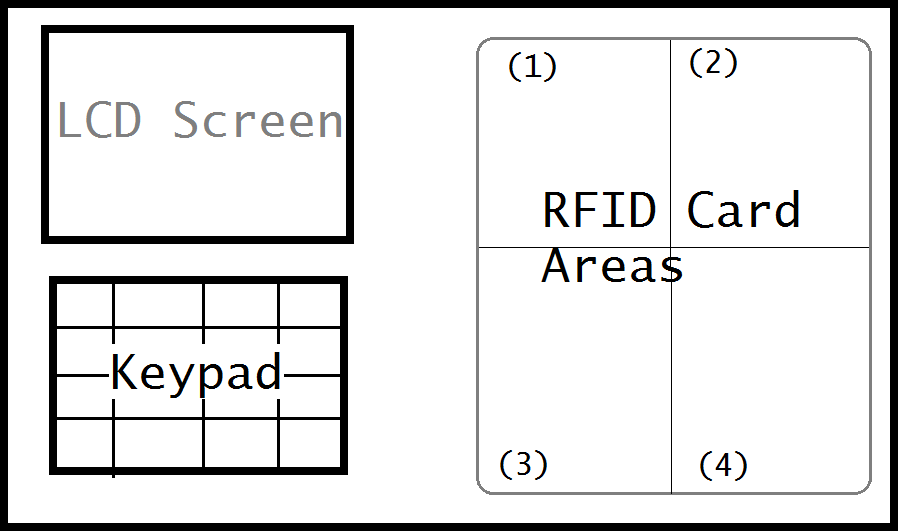
\includegraphics[width=0.6\textwidth]{images/exampleFrontPanel.png}
	\caption{An example front panel layout for the system}
	\label{fig:exampleFrontPanel}
\end{figure}

\subsubsection{Functional Requirement}

The system must support the following modes of operation:

\begin{description}
	\item[Single Player:] Allows the user to select from, and play, single player
		games. Upon entering Single Player mode, the system prompts the user to
		select a game to play from those stored in memory. Selecting a valid game
		loads the game from memory and begins game execution.
	\item[Multiplayer:] Allows the user to select and play multiplayer games.
		Upon entering Multiplayer mode, the system activates wireless communication
		and attempts to connect to other users in Multiplayer mode. Once a
		connection is established, the users select a multiplayer game on both
		systems and gameplay begins.
	\item[Build Card:] Allows the user to create custom cards for a game. To
		create a custom card, the user will input the data via the keypad. The data
		stored will vary based on game requirements. All cards must contain unique
		card serial numbers or identifing ID numbers, and a code that specifies
		which games the card is valid for.
\end{description}

In all three modes, the user will be instructed by the programmed game to place
a card in the RFID reading area to interact with the game and control events. 

\subsubsection{Operating Requirements}

The system must operate in a standard commercial or household environment. The system must be portable, wearable on the user's arm, and operate on an internal power supply.

\subsubsection{Reliablility and Safety Requirements}

The system must be compliance with communication and electromagnetic radiation
standards including those from the U.S. Federal Communication Committee, and
applicable state and federal child safety laws.

\subsection{Identified Use Cases}\label{sec:identifiedUseCases} % Alyanna

The user interacted with the system through the game. In the figure below, a user would interact with the system through single player,
multiplayer, or build card mode. In a single player game, the user would play against a computer. In a build card game, the user would be working
with the system to create/modify cards. Should a user be in multiplayer mode, they would interact with another using using the system during gameplay.

\subsection{Detailed Specifications}\label{detailedSpec} % Ryan

\subsection{Functional Decomposition}\label{functions} % Patrick

\section{Hardware Implementation}\label{hwImplementation} 

\subsection{Top Level Design}\label{hwTopLevel} % Patrick

\subsection{Low Level Design}\label{hwLowLevel} % Patrick

\section{Software Implementation}\label{swImplementation}
%
%What is your design????
%
%Present your design starting from a top level functional view and potentially
%block diagram or high level architecture.  Refine that view to present and
%explain each of the modules that comprise the major functional blocks.
%Discuss
%the flow of control through the design.  Identify and discuss the specific
%processes/tasks you have implemented in your design. Explain your design
%choices.    

\subsection{Top Level Design}\label{swTopLevel} % Alyanna
%
%Put stuff here about the functional decomposition, system architecture,
%interaction of parts.

The software implementation for the RFID interaction suite consisted of developing the game for a user to play \(and for the developers to test\). The system took input from the Xbee, RFID tags, and keyboard. Data would be outputted through the LCD screen. Below is a figure depicting the overall software for the RFID interaction suite. 

\begin{figure}[H]
	\centering
	\includegraphics[width=\textwidth]{images/funDecomp.png}
	\caption{Software functional decomposition showing the major functional divisions and tasks}
	\label{fig:funDecomp}
\end{figure}

\begin{itemize}
	\item Play Game
		\begin{itemize}
			\item Load Game: The program would have to load the correct game based off of user input through the keypad. The system is told which game to select based off of a set flag.
			\item Execute Game: After a game flag has been set, the game would run until a player has finished.
		\end{itemize}
	\item Read/Write Cards
		\begin(itemize)
			\item Scan for New Cards: During game mode or build card mode, the system would scan for new cards via the RFID reader/writer.
			\item Write Card: During the "build card" part of the game, the user would be able to write data to the cards through the RFID reader/writer. The user would have the ability to add a name and attack moves to the card through the external keypad and the in-game keyboard.
			\item Read card: During game mode, the system would check for available cards to work with. If a player was in the middle of a duel, the system would scan for new cards to use for gameplay. If a reader was trying to build new cards, the system would look for available cards to be modified.
		\end(itemize)
	\item Access Database
		\begin(itemize)
			\item Read Data to SRAM: Reads game-relevent data. For example, when a game is to be loaded, the system load the game from the SRAM. Or if the computer were to read in a monster during a single player duel game, it would access the database of monsters.
			\item Write Data to SRAM: Writes new game data. If new monsters or games were to be added to the system, it would be written to the SRAM for future use.
			\item Look Up / Reference Table: Used as a reference for memory locations of data in the SRAM \(i.e. ''Phone book''\).
		\end(itemize)
	\item External Communication
		\begin(itemize)
			\item RS232 Driver: The back end of the system uses the USART to communicate with the Xbee wireless chips and RFID drivers. Information was sent out or recieved by the system through these peripherals.
			\item Wireless Driver: In addition to the RS232, a driver for the Xbee wireless had to be implemented to allow the system to communicate with other users during the multiplayer game.
		\end(itemize)	
	\item User Interaction
		\begin(itemize)
			\item Read Keypad: A driver was made to read key presses from the user. Different parts of the system could read the keypad using functions built in this driver.
			\item Display: An LCD driver was modified to develo
			\item Card Reaction: An LED driver was made to control the LED lights of the RFID interaction suite. This would indicate to the user whether a card had been properly registered or not, based off of the color of the lights.
		\end(itemize)
\end{itemize}


\subsection{Low Level Design}\label{swLowLevel} % Alyanna
%
%task level implementation details here. Control diagram goes here, etc.



A major software component of the RFID interaction suite were the built in games.

\begin{itemize}
	\item LCD.c and LCD.h
		\item The majority of documentation for our ST7735 1.8 TFT LCD screen did not include example code for how to use the screen. Most tutorials or example code \(i.e. Adafruit\) assumed that the user would be programming on an Arduino UNO, which had built in libraries for fonts and shapes. The link below features code found on Google which interfaces the LCD with a PIC microcontroller using the chip's SPI function. However the code was not optomized, thus LCD.c and LCD.h are modified versions of the code. The original drawBox function in LCD.c created a box pixel by pixel - it would take a beginning pixel location and an ending pixel location, causing load times to take longer. The new box function takes the beginning and end coordinates for the box and fills everything in between by printing out pixels all at once. Another function printrs was made to take a char pointer to a string and print it out on the LCD. A major advantage to using this example code was that it already built a font library for the LCD screen. Had the group not utilized this, they would have taken time defining the pixel structure for every possible character. 
		\item Original Code (unmodified): https://sites.google.com/site/arduinomega2560projects/microchip-pic/level-3/st7735-1-8-tft
	\end {itemize}

% Insert State Machine for Game Here	
	
\begin{itemize}
	\item Game.c and Game.h
		\begin{itemize}
			\item Game.h was a header file which defined the following structures for running the game:
				\begin(itemize)
					\item Types: This structure defined element types for card monsters, which was indicated by an integer.
						\begin{itemize}
							\item Fire Type\= 0
							\item Water Type \= 1
							\item Earth Type \= 2
						\end
					\item Move: Each card had a set of attack moves to be used during the card duel game. This structure defines characteristics for each move, which can be modified by the user during the build card mode.
						\begin{itemize}
							\item char moveName\[9\] \= A nine character array which would store the name of a move/
							\item Type moveType \= Element type of the move, which can be fire, water or earth. Different move types have more damage against opposite elements. For example, a fire type is hurt more by a water type attack, etc.
							\item int baseDamage \= The maximum amount of possible damage for the move
							\item int uses \= Number of times a move can be used - during game mode, this number decreases as the same move is used. Once it hits 0, a user can no longer us the same attack.
						\end
					\item Monster: Each card represented a particular monster that could be selected during the game.
						\begin{itemize}
							\item char monsterName\[9\] \= Customizable name for the card, defined by the user.
							\item int monsterID \= A unique ID for a card; standardizes the card so the system can look it up quickly, despite what custom name is. Cannot be modified by user.
							\item int level \= Level of the monster, used for determining the success rate of an attack, talked about more in the pickMove function.
							\item Type monsterType \= Element type of the monster, relevant during game play mode. If a monster is hit with an attack of the opposite element \(ex. fire and water), then the monster will take more damage because of it's type.
							\item Move movelist \= An array that held how many moves were available in the card. Each card had a maximum of 3 moves.
						\end
					\item gameData:
						\begin{itemize}
							\item int myScore \= User's score; beginning score is 100. Updated as user experiences an attack from an opponent.
							\item int oppScore \= Opponent's score; beginning score is 100. Updated as user executes a successful attack.
							\item short turn \= Keeps track of who's turn it is during the game
							\item int gameOver \= Checks current game status, a 1 meant the game was over while 0 meant the game was still happening
							\item int monSel \= Selected card defined by user
							\item int moveSel \= Selected move defined by user
							\item Monster* myMonster\= A pointer to the monster that has been selected - enables access for all its traits as defined by the monster structure, like name, move, etc.
							\item Move* myMove \= User's selected attack to be used during their turn
							\item Move* oppmove\= Opponent's move received by the user during the opponent's turn
							\item char name\[5\] \= Name of the user playing during a game; this is defined during the initial execution of a game and is selected through a software keyboard
						\end
					\item Additionally, all functions in game.c have access to globalData which is shared among all components.
				\end
			\item Single Player: Single player mode followed the direction of the state machine diagram. Gameplay is as follows:
					\begin{enumerate}
						\item At the start of a game, the system randomly picks who goes first - the user or the computer. Afterwards, it would read in whatever cards through the getCard function, so that monsters are available for the player to use. If it is the user's first time playing, the system will prompt the user to enter a name using the processKeyboard helper function. This name would then be stored in gameData -> name.
						\item During the user's turn, they would select a card to play and pick a move to attack their opponent. This is done in the selectCard and pickMove helper functions, updating monSel, moveSel, and myMove in gameData. The effectiveness of the attack is based off of the monster level, and the total amount of damage of the attack is based off of the element. 
						\item Once the total damage has been determined, the game would then subtract this amount from the oppScore in gameData, and the display would be updated to reflect the change. 
						\item When it was not the user's turn, the user would wait for the computer to randomly select a move, thus modifying oppMove. The computer has access to all monsters that have been loaded on the SRAM, thus having access to all sorts of attacks. The success rate of the attack is also randomized, so it is possible for the computer to miss. All random variables were seeded to a software system timer on the PIC to ensure random numbers occurred every time it was called.
						\item However, if an attack was successful, the total amount of damage would be subtracted from myScore and the LCD display would update.
						\item During every game, helper function gameStatus was called to check whether the game was over. It compared the oppScore and myScore to 0, and if either of them were equal it would change gameOver in game data to equal 1, indicating someone lost.
						\item  Once game was over, printResults would be executed to display the results of the game, based off of the scores.
			\item Multiplayer: Structure of gameplay is essentially the same as single player, however instead of playing against a computer, the opponent is another player using a seperate system. Thus the following changes are made:
					\begin(enumerate)
						\item At the start of the game, the user would be given the option of hosting a game or finding a game to join. The temporary variable hostOrFind would indicate 0 for hosting a game or 1 for finding a game to join.
						\item The system would then set up the Xbee to either host a game or join a game using the setupXbee helper function, thus establishing a connection with the user. 
						\item Once a connection was made, game play would continue like single player mode. 
						\item During the user's turn, they would have to send moves over Xbee to the player, and receive the resulting score from the opponent. The recieved score would be stored in oppScore. 
						\item During an opponent's turn, the user would wait to receive a move over Xbee from the other player. Upon recieving it, the user would take damage based off of the element and level of the monster/move. The user would then update its myScore and send the new score over Xbee to the other player.
					\end
			% RYAN GO DO THIS
			\item Build Cards:
			\item Helper Functions:
				\begin{itemize}
					\item selectCard: 
					\item pickMove: Similar to selectCard, pickMove showed the user what attack moves were available based off of the selected card.
					\item processKeyboard: Since the 4x4 keypad was limited in options for characters, a software keyboard was created. Users could scroll through the characters on the screen using the external keypad and enter a 5 character string. Characters were selected based off of the position of the cursor and added to an empty string called names\[\] - when the system read a \# from the keypad, it would add a backslash 0 to indicate the array was a string. This keyboard was used for creating a player name or customizations on in the build card interface.
					\item Print Functions: Many print functions were created to print different screens for the game using functions from LCD.c. For example, printSelect printed out the menu for selecting cards while printGame printed the current game status, showing off the scores and turns.
				\end{itemize}
		\end{itemize}
		
		
		\item keypadDriver.c and keypadDriver.h
		
		\item
\end{itemize}


\section{Presentation, Discussion, and Analysis of the Results}
%
%Based upon the execution of your design, present your results. Explain them
%and
%what was expected, and draw any conclusions (for example, did this prove your
%design worked).
%
%In addition to a detailed discussion and analysis of your project and your
%results, you must include all the answers to all questions raised in the lab.
\subsection{Results } % Ryan

\subsection{Discussion of Results } % Alyanna

\subsection{Analysis of Any Errors } % Ryan
%
%This one is obvious. Do this section as appropriate.  If it improves the flow,
%it does not need to be a separate section and may be included in the
%presentation, discussion, and analysis of the results.  However, it will still
%be graded separately and must be present.

The biggest problem with the final version of this project that was present at
demo time was the fact that the multiplayer features were not implemented.
There was test code that correctly configured the Xbee modules for multiplayer,
but they were not completely implemented with the game.  The reason for this
was because when the $I^2C$ system was implemented, the entire game had to be
modified to run within the scheduler, when it was just a single function
before.  $I^2C$ communication is controlled by the system's interrupt handler,
and certain flags are set depending on whether data is being sent or received.
Those flags have to be processed, and a game that is running in a function and
taking control of the entire system would not allow for those flags to be
processed.  The time it took to port the game over to running completely within
the scheduler made it impossible to get the multiplayer functions completely
implemented and working in time.

Another problem at the time of the demo was that card reading was not 100\%
functional.  The system had four distinct sets of data that could be
successfully written to a card using the ``Build Cards'' option from the
system's main menu, but the data was not being displayed properly in the
singleplayer game.  Data coming from the card over the $I^2C$ connection was
confirmed to be correct, but the game was not interpreting and displaying the
information correctly to the user.  This was also a matter of running out of
time.  For the same reasons as above (converting the game to be run within the
flag-based scheduler) the RFID reading still had some kinks to work out at the
time of the demo.  Those problems were that:

\begin{itemize}
	\item Monster type was being read incorrectly
	\item Monster name was being displayed incorrectly
	\item Complete attack list was not implemented
\end{itemize}

For demo purposes, only the first attack would be read and it would be copied
to all three attack slots.  Only the ``FAIL'' attack ID was programmed to be
read, and if the ID did not match the ``FAIL'' attack's ID, then it was
interpreted as a ``SCRATCH'' attack.  This function worked correctly, but the
rest of the attack IDs were not implemented.  The monster's level was correctly
read as well.

Finally, there was an error when finishing a singleplayer game.  When the game
was complete, the main menu was not being properly displayed.  Once again, the
problem was time, and the main menu's controls were still functional.  Another
menu could be loaded by navigating the invisible menu and choosing an option,
letting that screen load, and then pressing the ``B'' key to return back to the
main menu and redraw it.

\subsection{Analysis of Implementation Issues and Workarounds} % Patrick
%
%State any problems you encountered while working on the project. If your
%project did not work or worked only partially, provide an analysis of why and
%what efforts were made to identify the root cause of any problems. \\
%

\section{Test Plan } % Ryan
%
%Overall summary of what needs to be tested to ensure that your design meets
%the
%original requirements, 2-3 paragraphs maximum unless specified otherwise

\subsection{Test Specification} % Patrick
%
%Annotated description of what is to be tested and the test limits.  This
%specification quantifies inputs, outputs, and constraints on the system.  That
%is, it provides specific values for each. 
%
%Note, this does not specify test implementation...this is what to do, not how
%to do it.

\subsection{Test Cases} % Alyanna
%
%Annotated description of how your system is to be tested against the test
%limits
%Note, this does specify test implementation...this is not what to do, this is
%how to do it based upon the test specification.




\section{Summary and Conclusion}
%
%You should know these sections very well, no need to explain.  Note, however,
%that they are two different sections.  The summary is just that, a summary of
%your project.  It should loosely mirror the abstract with a bit more detail.
%The conclusion concludes the report, potentially adds information that is
%often
%outside the main thrust of the report, and may offer suggestions or
%recommendations about the project.

\subsection{Final Summary}


\subsection{Project Conclusions} % Patrick, Alyanna, Ryan
% Include comments and reflections on the capstone. What went well, what could
% be improved next time, What was enjoyable and/or challenging.

This project had many hardware components that were new to the group. There was little documentation to gooff of and previous capstone projects had not done anything similar to our design requirements. Much of the project was spent
reading documentation and figuring out how to design drivers compatible with the PICs, since most available documentation was
for Arduinio shields. Using the LCD and Xbee was more difficult since online tutorials referenced the Arduino shield. RFID tags
were a completely new piece of hardware to work with with little documentation that the group had to contact the company for help.

With all this new technology, the group broke down building and testing into separate components. The intention was to put everything
together at the end and make a scheduler to fire off every function at a particular time. This was the first development flaw - assuming
everything would work when put together. There was miscommunication over how the scheduler would work that many functions with while 
loops had to be redone using flags. A better method would have been to consistently putting components together once their functionality
was verified separately. Additionally, another PICKit 3 should have been bought for use during testing - with only one PICKit, components
had to be tested and debugged one at a time after programming. The ability to consistently load the program into PICs and observe the results
would have reduced the time for debugging and testing each individual part.

The original intent of the project was to have a working motor that would move the
RFID reader to read multiple cards. Another feature was that he user would also be able to make custom cards
with their own ID, attack names, moves, and type. Due to time constraints and testing, these idea had
to be scrapped in the final implementation. Future implementations should include these features.

\pagebreak
\appendix


\section{Breakdown of Lab Person-hours (Estimated)}
% Use the '&' to separate columns
\begin{tabular}{|l|*{4}{r|}}
	\hline
	Person & Design Hrs & Code Hrs & Test/Debug Hrs & Documentation Hrs \\ \hline
	Patrick & x & x & x & x  \\ \hline
	Alyanna & x & x & x & x \\ \hline
	Ryan & x & x & x & x  \\ \hline
\end{tabular}

~\\

By initializing/signing above, I attest that I did in fact work the
estimated number of hours stated. I also attest, under penalty of shame,
that the work produced during the lab and contained herein is actually my
own (as far as I know to be true). If special considerations or
dispensations are due others or myself, I have indicated them below.

\pagebreak

\section{Bill of Materials\label{appendix:bom}}
Table~\ref{tab:bomTable} lists the bill of materials for the construction of
one system.

\begin{table}[h]
	\begin{tabular}{llll}
		\multicolumn{4} {c} {\textbf{Bill of Materials}} \\
		\toprule
		\textbf{Item}                         & \textbf{Unit Cost} & \textbf{Quantity} & \textbf{Total Cost} \\ \midrule
		TI HI-Plus RFID Tags                  & 0.91          & 20                & 18.20               \\
		DLP-RFID2 RFID Reader/Writer          & 50            & 3                 & 150                 \\
		Xbee S1 Wireless Chips                & 30            & 2                 & 60                  \\
		PLA Makerbot Filament                 & 48            & 1                 & 48                  \\
		GAL22V10D                             & 3.5           & 4                 & 14                  \\
		PICKit 3                              & 45            & 2                 & 90                  \\
		CY7C128A SRAM                         & 4             & 2                 & 8                   \\
		3.3 Volt Linear Regulator             & 3.22          & 2                 & 6.44                \\
		Lever Switch, micro SPDT, momentary   & 2.5           & 6                 & 15                  \\
		16-key Numeric Keypad                 & 7.5           & 2                 & 15                  \\
		128x169 Color LCD                     & 17            & 2                 & 34                  \\
		PIC18F46K22 Microcontrollers          & 7.7           & 4                 & 30.8                \\
		RGB LED, Common Cathode               & 4             & 8                 & 12                  \\
		(EXTRA)                               &               &                   &                     \\
		(EXTRA)                               &               &                   &                     \\
		(EXTRA)                               &               &                   &                     \\ \bottomrule
		Total Cost                            &               &                   &                    
	\end{tabular}
	\caption{\label{tab:bomTable}}
\end{table}

%\FloatBarrier
%\section{Hardware Diagrams\label{appendix:hwDiagrams}}
%\begin{figure}[H]
%	\centering
%	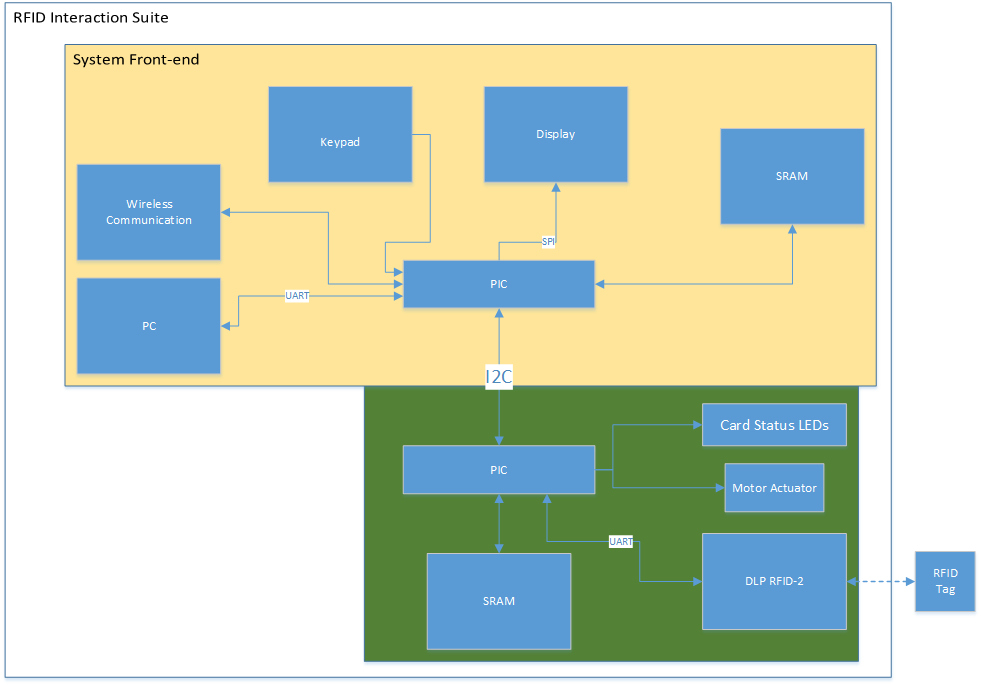
\includegraphics[width=\textwidth]{images/BlockDiagram.png}
%	\caption{High level block diagram of the system hardware components}
%	\label{fig:highLevelBlockDiagram}
%\end{figure}
%
%\begin{figure}[H]
%	\centering
%	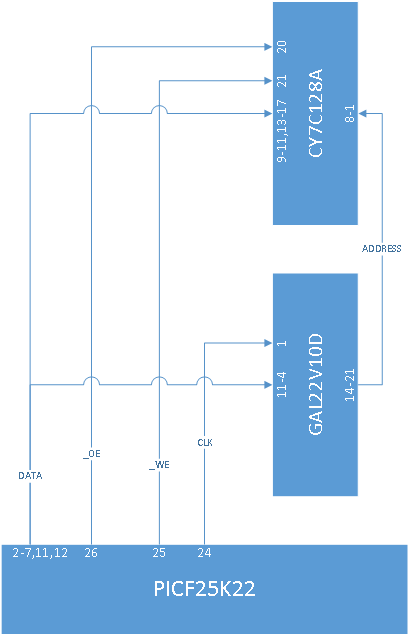
\includegraphics[width=0.8\textwidth]{images/SRAMHardwareBlock.png}
%	\caption{Block diagram of the SRAM hardware system}
%	\label{fig:sramBlockDiagram}
%\end{figure}
%
%\begin{figure}[H]
%	\centering
%	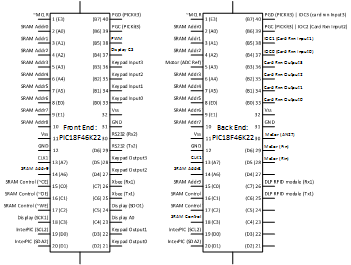
\includegraphics[height=4in]{images/PinOuts.png}
%	\caption{Pinouts to the front- and back-end microcontrollers}
%	\label{fig:pinoutDiagram}
%\end{figure}
%
%\FloatBarrier
%\section{Functional Decomposition Diagram\label{fig:funcDecomp}}
%
%\begin{figure}[H]
%	\centering
%	\includegraphics[width=\textwidth]{images/funDecomp.png}
%	\caption{Software functional decomposition showing the major functional
%	divisions and tasks}
%	\label{fig:funDecomp}
%\end{figure}
%
%\FloatBarrier
%\section{State Diagrams}
%\FloatBarrier
%\subsection{System State Diagram\label{fig:sysStateDiagram}}
%\begin{figure}[H]
%	\centering
%	\begin{subfigure}{0.48\textwidth}
%		\includegraphics[width=\textwidth]{images/overallSystemDiagram.png}
%		\caption{}
%		\label{fig:sysStates}
%	\end{subfigure}
%	~
%	\begin{subfigure}{0.48\textwidth}
%		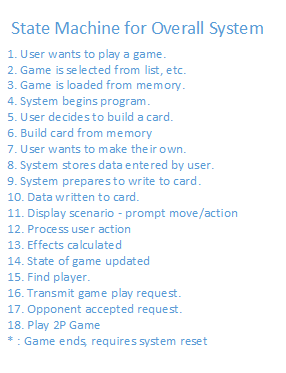
\includegraphics[width=\textwidth]{images/OSStates.png}
%		\caption{}
%		\label{fig:statesLegend}
%	\end{subfigure}
%	\caption{State diagram of the primary operating system.
%		Figure~\ref{fig:sysStates} shows the states while
%		Figure~\ref{fig:statesLegend} provides a legend}
%		\label{fig:systemStateDiagram}
%	\end{figure}
%
%	\FloatBarrier
%	\subsection{General Gameplay State Diagram\label{appendix:gameplayDiagram}}
%	\begin{figure}[H]
%		\centering
%		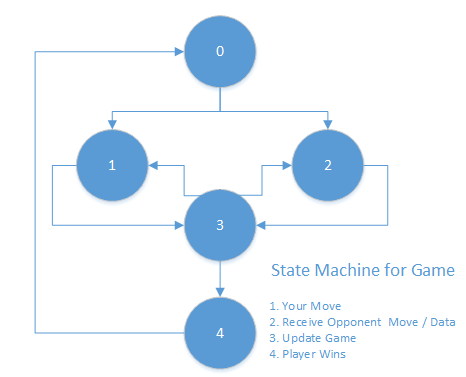
\includegraphics[width=\textwidth]{images/gamePlayState.png}
%		\caption{State diagram of basic turn-based game}
%		\label{fig:gamePlayState}
%	\end{figure}
%
%	\FloatBarrier
%	\section{Control Flow Diagrams}
%
%	\begin{figure}[H]
%		\centering
%		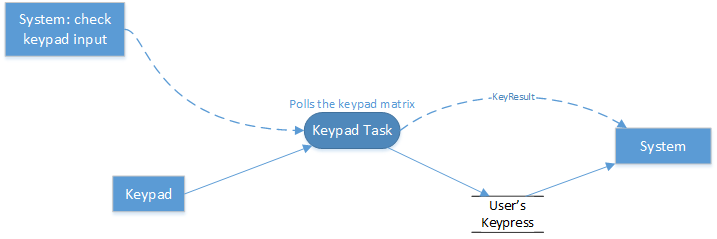
\includegraphics[width=0.75\textwidth]{images/keypadDataFlow.png}
%		\caption{Keypad response}
%		\label{fig:keypadDataFlow}
%	\end{figure}
%
%	\begin{figure}[H]
%		\centering
%		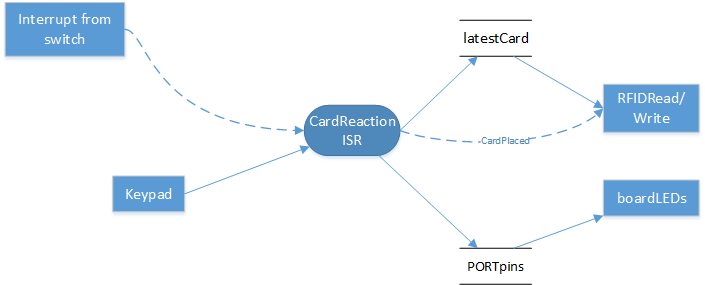
\includegraphics[width=0.8\textwidth]{images/reactionDataFlow.png}
%		\caption{Card Reaction LEDs}
%		\label{fig:cardReactionDataFlow}
%	\end{figure}
%
%	\begin{figure}[H]
%		\centering
%		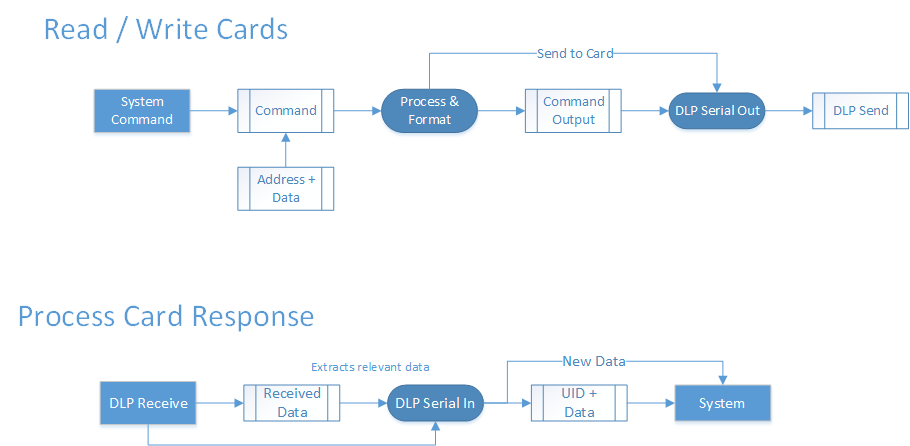
\includegraphics[width=0.8\textwidth]{images/RFIDreaderDataFlow.png}
%		\caption{RFID tag reader subsystem}
%		\label{fig:rfidDataFlow}
%	\end{figure}
%
%	\begin{figure}[H]
%		\centering
%		\begin{subfigure}{\textwidth}
%			\includegraphics[width=\textwidth]{images/I2CReceiveDataCtrlFlow.png}
%			\caption{}
%			\label{fig:i2cReceiveFlow}
%		\end{subfigure}
%
%		\begin{subfigure}{\textwidth}
%			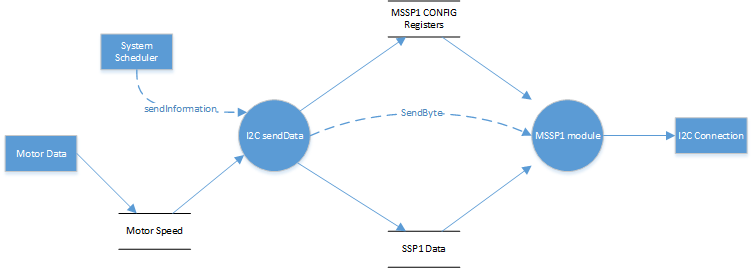
\includegraphics[width=\textwidth]{images/I2CSendCtrlFlow.png}
%			\caption{}
%			\label{fig:i2cSendFlow}
%		\end{subfigure}
%		\caption{I2C communication between microcontrollers.
%		Figure~\ref{fig:i2cReceiveFlow} shows the flow for received data and
%		Figure~\ref{fig:i2cSendFlow} shows the flow for transmitted data.}
%		\label{fig:i2cCtrlFlow}
%	\end{figure}
%
%	\FloatBarrier
%	\section{Project Schedule\label{appendix:ganttChart}}
%	\begin{figure}[h]
%		\centering
%		\begin{adjustbox} {rotate=90,center}
% 		
\includegraphics[height=0.7\textwidth]{images/NewGantt.png}
% 	\end{adjustbox}
% 	\caption{Project Gantt Chart}
% 	\label{fig:ganttChart}
% \end{figure}
%
%	\clearpage
%	\section{Source Code}
% We will put code here. Use the format:
%    \subsection{Main Function}
%%    \lstinputlisting{../code/main.c}
%%
%%    \subsection{Tasks}
%%    \subsubsection{Task Control Blocks}
%%    \lstinputlisting{../code/tcb.h}
%	Source code for this project is provided below.
%
%	\subsection{System Scheduler}
%	The system-wide global definitions and variables are also given here for
%	convenience.
%	\lstinputlisting{../FrontEnd.X/globals.h}
%	\lstinputlisting{../FrontEnd.X/interrupts.h}
%	\lstinputlisting{../FrontEnd.X/SchedMain.c}
%
%	\subsection{Creating Cards}
%	\lstinputlisting{../FrontEnd.X/buildCard.c}
%
%	\subsection{Example Game}
%	Both a single player and multiplayer version of the same game are provided.
%	\lstinputlisting{../FrontEnd.X/game.h}
%	\lstinputlisting{../FrontEnd.X/game.c}
%
%	\subsection{I$^2$C InterPIC Communication}
%	\lstinputlisting{../FrontEnd.X/i2cComm.h}
%	\lstinputlisting{../FrontEnd.X/i2cComm.c}
%
%	\subsection{Keypad Driver}
%	\lstinputlisting{../FrontEnd.X/keypadDriver.h}
%	\lstinputlisting{../FrontEnd.X/keypadDriver.c}
%
%	\subsection{LCD Driver}
%	\lstinputlisting{../FrontEnd.X/LCD.h}
%	\lstinputlisting{../FrontEnd.X/LCD.c}
%
%	\subsection{Card Reaction Control}
%	\lstinputlisting{../FrontEnd.X/LED.h}
%	\lstinputlisting{../FrontEnd.X/LED.c}
%
%	\subsection{Motor Driver}
%	\textit{Note: This feature was not implemented in the final product}
%	\lstinputlisting{../FrontEnd.X/motorDriver.h}
%	\lstinputlisting{../FrontEnd.X/motorDriver.c}
%
%	\subsection{RFID Reader Driver}
%	\lstinputlisting{../FrontEnd.X/rfidReader.h}
%	\lstinputlisting{../FrontEnd.X/rfidReader.c}
%
%	\subsection{EIA-232 Serial Connection}
%	\lstinputlisting{../FrontEnd.X/rs232.h}
%	\lstinputlisting{../FrontEnd.X/rs232.c}
%
%	\subsection{SRAM Primary Memory}
%	\textit{Note: There are two different files for each microcontroller due to
%	hardware configurations}
%	\lstinputlisting{../FrontEnd.X/SRAM.h}
%	\lstinputlisting{../FrontEnd.X/SRAMfront.c}
%	\lstinputlisting{../FrontEnd.X/SRAMback.c}
%
%	\subsection{SPI Initialization}
%	\textit{Note: SPI used for communication with the LCD display}
%	\lstinputlisting{../FrontEnd.X/startup.h}
%	\lstinputlisting{../FrontEnd.X/startup.c}
%
%	\subsection{Wireless Connectivity via Xbee}
%	\lstinputlisting{../FrontEnd.X/xbee.h}
%	\lstinputlisting{../FrontEnd.X/xbee.c}
%
	\end{document}
